% ═══════════════════════════════════════════════════════════════════════════════
% Transformer Tomography: Characterizing Weight Identifiability Limits
% from Black-Box Logit Access
% NeurIPS 2026 Submission
% ═══════════════════════════════════════════════════════════════════════════════
\documentclass{article}

% NeurIPS 2026 style
\usepackage[final]{neurips_2026}

% ── Packages ─────────────────────────────────────────────────────────────────
\usepackage[utf8]{inputenc}
\usepackage[T1]{fontenc}
\usepackage{hyperref}
\usepackage{url}
\usepackage{booktabs}
\usepackage{amsfonts}
\usepackage{amsmath}
\usepackage{amssymb}
\usepackage{amsthm}
\usepackage{nicefrac}
\usepackage{microtype}
\usepackage{xcolor}
\usepackage{graphicx}
\usepackage{subcaption}
\usepackage{algorithm}
\usepackage{algorithmic}
\usepackage{multirow}
\usepackage{wrapfig}
\usepackage{mathtools}

% ── Theorem environments ─────────────────────────────────────────────────────
\newtheorem{theorem}{Theorem}
\newtheorem{proposition}[theorem]{Proposition}
\newtheorem{lemma}[theorem]{Lemma}
\newtheorem{corollary}[theorem]{Corollary}
\newtheorem{definition}[theorem]{Definition}
\newtheorem{remark}[theorem]{Remark}

% ── Custom commands ──────────────────────────────────────────────────────────
\newcommand{\R}{\mathbb{R}}
\newcommand{\E}{\mathbb{E}}
\newcommand{\cQ}{\mathcal{Q}}
\newcommand{\cL}{\mathcal{L}}
\newcommand{\cG}{\mathcal{G}}
\newcommand{\cS}{\mathcal{S}}
\newcommand{\cT}{\mathcal{T}}
\newcommand{\cO}{\mathcal{O}}
\newcommand{\btheta}{\boldsymbol{\theta}}
\newcommand{\bphi}{\boldsymbol{\phi}}
\newcommand{\bz}{\mathbf{z}}
\newcommand{\bh}{\mathbf{h}}
\newcommand{\bx}{\mathbf{x}}
\newcommand{\bW}{\mathbf{W}}
\newcommand{\bJ}{\mathbf{J}}
\newcommand{\bG}{\mathbf{G}}
\newcommand{\bV}{\mathbf{V}}
\newcommand{\bU}{\mathbf{U}}
\newcommand{\bI}{\mathbf{I}}
\newcommand{\norm}[1]{\left\lVert #1 \right\rVert}
\newcommand{\inner}[2]{\langle #1, #2 \rangle}
\DeclareMathOperator{\tr}{tr}
\DeclareMathOperator{\diag}{diag}
\DeclareMathOperator{\rank}{rank}
\DeclareMathOperator{\SiLU}{SiLU}
\DeclareMathOperator{\RMSNorm}{RMSNorm}

% ═══════════════════════════════════════════════════════════════════════════════
\title{Transformer Tomography: Characterizing Weight Identifiability Limits\\from Black-Box Logit Access}

\author{
  Anonymous Authors
}

\begin{document}
\maketitle

% ═════════════════════════════════════════════════════════════════════════════
% ABSTRACT
% ═════════════════════════════════════════════════════════════════════════════
\begin{abstract}
We study a fundamental question in LLM security: \emph{how much of a transformer's internal weight structure is identifiable from black-box logit access?}  Prior work has shown that the output projection layer can be algebraically extracted from API queries, but whether this extends to internal layers is unknown.  We address this through \textbf{Transformer Tomography}, a principled framework grounded in observability theory.  Our key theoretical contribution is the \emph{suffix observability Gramian}, $\bG(\cQ) = \frac{1}{N}\sum_{i=1}^{N}\bJ_i^\top\bJ_i$, defined on the \emph{symmetry-quotiented} parameter space, which characterizes which parameter directions are locally identifiable from a given query set.  We derive the continuous symmetry group of modern transformer architectures (RMSNorm scale absorption, gated-MLP neuron scaling) and show that projecting out the gauge null-space is necessary for meaningful identifiability analysis.  Building on this theory, we propose \textbf{S-PSI} (Sensitivity-Guided Progressive Suffix Inversion), combining algebraic initialization via sketched Gauss--Newton in the observable subspace, logit-sensitivity matching, and gauge-projected optimization.  In a controlled case study on Qwen2.5-0.5B (494M parameters), we find a \textbf{negative identifiability result} with a nuanced structure: (i)~the projected Gramian is \emph{observation-dependent}---with $K{=}8$ suffix positions, the sketched rank is $\approx 32$, but expanding to $K{=}128$ positions yields \emph{full rank} with well-conditioned spectra ($\kappa \approx 2.4$) and eigenvalues scaling linearly with $K$; (ii)~the next-deeper block (Block~22) appears unobservable under oracle boundary injection (which replaces its output), but an independent diagnostic without boundary injection reveals it has \emph{stronger} signal than the last block; (iii)~despite full-rank, well-conditioned Gramians, no initialization strategy recovers any weight matrix ($\cos \approx 0.12$--$0.14$, consistent with initialization bias)---only RMSNorm parameters recover ($\cos \approx 0.67$--$0.99$).  This reveals that \emph{sampled observability is necessary but not sufficient}: the sketched Gramian confirms that at least 128 parameter directions are observable from logit queries, but gradient-based optimization in the full $14.9 \times 10^6$-dimensional space remains trapped near initialization.  Functional evaluation shows oracle-regime models achieve KL~$0.42$ ($24\times$ better than random) despite zero parameter recovery, but this appears only with oracle boundary states and may reflect standard knowledge-distillation dynamics.  For the architecture, scale, and passive-query regime studied here (Qwen2.5-0.5B, natural-text queries, gradient-based optimization), these findings provide strong evidence that sampled observability alone does not translate into parameter recovery for internal transformer layers, while the Gramian framework provides a precise, observation-dependent diagnostic for parameter exposure.  Whether this gap persists at larger scales, with different architectures, or under actively optimized queries remains an open question.
\end{abstract}

% ═════════════════════════════════════════════════════════════════════════════
% 1. INTRODUCTION
% ═════════════════════════════════════════════════════════════════════════════
\section{Introduction}
\label{sec:intro}

Large language models (LLMs) deployed as black-box APIs represent billions of dollars of investment in data curation, training compute, and algorithmic innovation. The security assumption underlying this deployment model is that API access --- which returns only output logits or token probabilities --- does not expose the model's internal parameters. But how valid is this assumption?

Recent work has begun to chip away at this barrier. \citet{carlini2024stealing} demonstrated that the output projection layer (\texttt{lm\_head}) of production LLMs can be \emph{algebraically extracted} from a modest number of API queries. \citet{tramer2016stealing} showed that simpler models are vulnerable to equation-solving attacks. However, a fundamental question remains unanswered:

\begin{quote}
\emph{How deep into a transformer's architecture can weight recovery extend, and what governs the boundary between identifiable and non-identifiable layers?}
\end{quote}

This question has profound implications. If internal transformer layers are identifiable from logits, the attack surface extends far beyond the output projection --- potentially exposing proprietary architectural innovations, fine-tuning data through weight inspection, or enabling perfect model cloning that circumvents API rate limits and usage policies.  Figure~\ref{fig:overview} provides a schematic overview of the problem and our findings.  We note that our identifiability analysis is necessarily \emph{query-dependent}: the Gramian characterizes identifiability with respect to a specific query distribution, and different (e.g., adversarially optimized) queries could in principle yield different observable subspaces.

\paragraph{This paper.} We formalize this question through the lens of \emph{observability theory} from control systems, adapted to the deep learning setting. Our central object is the \textbf{suffix observability Gramian}:
\begin{equation}\label{eq:gramian-intro}
    \bG(\cQ) = \frac{1}{|\cQ|}\sum_{\bx \in \cQ} \bJ_{\bx}^\top \bJ_{\bx},
\end{equation}
where $\bJ_{\bx} = \partial \bz / \partial \btheta_{\text{suffix}} \big|_{\bx}$ is the Jacobian of the logit output with respect to the suffix parameters, evaluated at query $\bx$. The eigenspectrum of $\bG(\cQ)$ --- computed on the \emph{gauge-projected} parameter space that quotients out continuous symmetries --- reveals precisely which parameter directions are identifiable from a given query set.

Building on this theoretical foundation, we develop \textbf{S-PSI} (Sensitivity-Guided Progressive Suffix Inversion), not primarily as an attack method, but as a \emph{diagnostic tool} that probes the boundary between identifiable and non-identifiable parameters in transformers.  S-PSI combines three techniques designed to maximize recovery potential:

\begin{enumerate}
    \item \textbf{Gauge-aware observability analysis.} We derive the complete continuous symmetry group of modern transformers (RMSNorm scale absorption $(\R_{>0})^d$ and gated-MLP neuron scaling $(\R_{>0})^{d_\text{ff}}$), construct its Lie algebra as a gauge basis, and project all analysis into the gauge-orthogonal complement. This is essential: without gauge projection, the Gramian would be rank-deficient even for perfectly identifiable parameters.

    \item \textbf{Algebraic initialization.} Rather than optimizing from random initialization, we solve a \emph{sketched Gauss--Newton} system in the observable subspace, providing a warm start that concentrates on identifiable parameter directions while avoiding gauge directions entirely.

    \item \textbf{Sensitivity matching.} Beyond matching logit values $\bz(\bx)$, we match logit \emph{responses} to input perturbations $\Delta\bz(\bx, \tilde{\bx}) = \bz(\tilde{\bx}) - \bz(\bx)$. This provides additional constraints that break symmetries inaccessible to logit matching alone.
\end{enumerate}

\paragraph{Contributions.}
\begin{itemize}
    \item We define the \emph{suffix observability Gramian} on gauge-quotiented parameter space and show it governs weight identifiability from logit access (\S\ref{sec:theory}).
    \item We derive the continuous symmetry group for RMSNorm + GatedMLP transformers and its gauge basis (\S\ref{sec:symmetry}).
    \item We prove a \emph{Gramian rank upper bound} via the hidden-dimension bottleneck and a \emph{depth-screening theorem} explaining why deeper blocks become unobservable (Theorems~\ref{thm:rank-bound}--\ref{thm:screening}), plus a Fisher information lower bound on query complexity (Remark~\ref{rem:fisher}).
    \item We develop S-PSI, combining algebraic initialization, sensitivity matching, and gauge-projected optimization (\S\ref{sec:method}).
    \item In a controlled case study on Qwen2.5-0.5B (494M parameters, 24 layers), we empirically show that the Gramian is \emph{observation-dependent}: with $K{=}8$ suffix positions the sketched rank is $\approx 32$, but expanding to $K{=}128$ yields full rank ($= k$) with eigenvalues scaling linearly in $K$ and condition number $\kappa \approx 2.4$---establishing that the Gramian bottleneck is in the observation window, not in the parameter structure.  Yet despite well-conditioned, full-rank Gramians, no initialization strategy recovers any weight matrix ($\cos \approx 0$ for all projections; block mean $\approx 0.12$--$0.14$ driven by LayerNorm).  This decoupling between \emph{observability} and \emph{recoverability} is our central empirical finding (\S\ref{sec:experiments}).
    \item We release our code and experimental artifacts for reproducibility.
\end{itemize}

\begin{figure}[t]
\centering
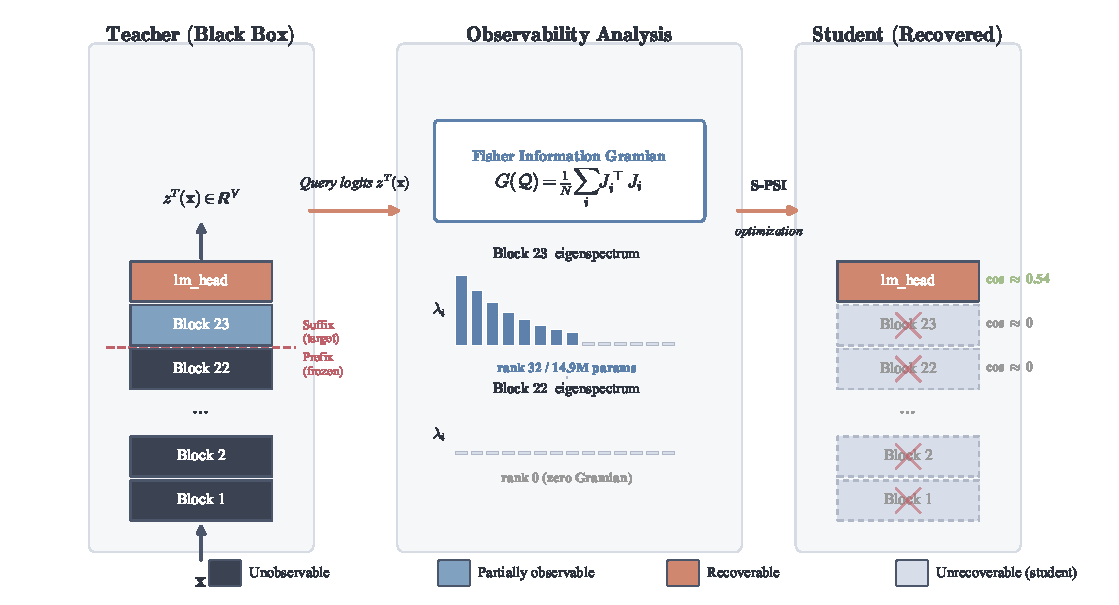
\includegraphics[width=\textwidth]{figures/framework_overview.pdf}
\caption{\textbf{Transformer Tomography overview} (Qwen2.5-0.5B case study).  We query a black-box teacher and analyze the suffix observability Gramian $\bG(\cQ)$ on gauge-quotiented parameter space.  The Gramian rank is observation-dependent: with $K{=}8$ suffix positions rank~$\approx 32$, expanding to $K{=}128$ yields full rank with $\sigma_{\max} \propto K$.  Despite full-rank, well-conditioned Gramians, no projection matrix is recovered ($\cos \approx 0$; block mean $\approx 0.14$ driven by LayerNorm)---revealing a gap between observability and recoverability.}
\label{fig:overview}
\end{figure}


% ═════════════════════════════════════════════════════════════════════════════
% 2. RELATED WORK
% ═════════════════════════════════════════════════════════════════════════════
\section{Related Work}
\label{sec:related}

\paragraph{Model extraction attacks.}
Model stealing has evolved from training surrogate models on query-response pairs \citep{tramer2016stealing} to functionally equivalent extraction \citep{jagielski2020high,orekondy2019knockoff}. \citet{carlini2024stealing} achieved a qualitative leap by showing that the final projection layer of production LLMs can be \emph{algebraically} recovered --- not merely approximated --- from a small number of crafted API queries. Their attack exploits the affine structure of the last-layer mapping $\bz = \bW_{\text{lm\_head}} \bh_N + \mathbf{b}$. However, they explicitly note that extending extraction beyond the output layer remains an open problem, as deeper layers lack this simple algebraic structure. Our work directly addresses this open question.

\paragraph{Knowledge distillation and model compression.}
Knowledge distillation (KD) \citep{hinton2015distilling,gou2021knowledge} trains a student to match teacher outputs but does not aim for \emph{parameter} recovery. The student learns a \emph{functionally equivalent} mapping, potentially with entirely different internal representations. Our setting is fundamentally different: we seek to recover the teacher's actual weight matrices, not merely its input-output behavior. This distinction matters for security analysis, intellectual property claims, and understanding model identifiability.

\paragraph{Neural network identifiability.}
Theoretical identifiability of neural networks has a rich history. \citet{sussmann1992uniqueness} showed that single hidden-layer networks with analytic activations are identifiable up to permutation symmetries. \citet{bui2020functional} extended this to deeper networks under specific conditions. For transformers, \citet{liu2025identifiability} recently studied identifiability of attention parameters. However, these works analyze identifiability \emph{in principle} (given infinite, noiseless observations) rather than \emph{in practice} from finite black-box queries. Our Gramian framework bridges this gap by quantifying identifiability as a function of the query set $\cQ$.

\paragraph{Observability in control theory.}
The observability Gramian is a classical tool in linear systems theory \citep{kailath1980linear}, characterizing which internal states can be inferred from output measurements. Extensions to nonlinear systems via empirical Gramians \citep{lall2002subspace} compute $\bG \approx \frac{1}{N}\sum_i \bJ_i^\top \bJ_i$ using Jacobians from perturbed trajectories. We adapt this framework to the novel setting of \emph{parameter} observability in deep networks, where the ``state'' is the weight vector and ``observations'' are logit outputs across queries.


% ═════════════════════════════════════════════════════════════════════════════
% 3. PROBLEM SETUP
% ═════════════════════════════════════════════════════════════════════════════
\section{Problem Setup}
\label{sec:setup}

\paragraph{Notation.}
Let $T$ denote a frozen teacher transformer with $L$ blocks, parameterized by $\btheta^T = (\btheta^T_1, \ldots, \btheta^T_L, \bW_{\text{lm\_head}}^T)$. The output logit mapping is $f_T: \bx \mapsto \bz^T(\bx) \in \R^{V}$, where $V$ is the vocabulary size. A student $S$ has identical architecture but parameters $\btheta^S$.

\paragraph{Threat model.}
The attacker has:
\begin{enumerate}
    \item \textbf{Black-box logit access}: can query $f_T(\bx)$ for arbitrary input sequences $\bx$.
    \item \textbf{Architecture knowledge}: knows the model class (e.g., Qwen2.5-0.5B) but not the weights.
    \item \textbf{Query budget}: total of $B$ API calls.
\end{enumerate}

\paragraph{Suffix decomposition.}
We partition the transformer into a \emph{prefix} (blocks $1, \ldots, L-K$) and a \emph{suffix} (blocks $L-K+1, \ldots, L$ plus \texttt{lm\_head}). The suffix parameters are $\btheta_{\text{suf}} \in \R^p$. For any input $\bx$, the prefix produces a boundary hidden state $\bh_{L-K}(\bx) \in \R^{d}$, and the suffix maps $\bh_{L-K} \mapsto \bz \in \R^V$.

\paragraph{Experimental regimes.}
We study two complementary settings:

\begin{itemize}
    \item \textbf{Boundary-state oracle} (upper bound on identifiability): The attacker receives the teacher's true boundary states $\bh^T_{L-K}(\bx)$ for each query. This isolates suffix identifiability from prefix error propagation.
    \item \textbf{Pure-logits} (realistic attack): The student's prefix is random-initialized and frozen. Only logits $\bz^T(\bx)$ are observed. This tests practical extraction limits.
\end{itemize}

The oracle regime establishes what \emph{could} be recovered under perfect conditions; the pure-logits regime reveals the practical gap introduced by prefix mismatch.


% ═════════════════════════════════════════════════════════════════════════════
% 4. THEORY: SYMMETRY AND OBSERVABILITY
% ═════════════════════════════════════════════════════════════════════════════
\section{Symmetry and Observability Theory}
\label{sec:theory}

\subsection{Continuous Symmetry Group of Transformers}
\label{sec:symmetry}

Modern transformers with RMSNorm and gated MLPs possess continuous symmetries that render the parameterization non-unique even when the input-output mapping is fully determined. We derive the complete symmetry group for architectures like Qwen and LLaMA.

\begin{definition}[Transformer symmetry group]
\label{def:symmetry}
The continuous symmetry group $\cG$ of a transformer block with RMSNorm and SiLU-gated MLP consists of:
\begin{enumerate}
    \item \textbf{RMSNorm scale absorption} $(\R_{>0})^d$: For each dimension $i \in [d]$, scaling the RMSNorm weight $g_i \mapsto \alpha_i g_i$ can be absorbed by the consumer weights $\bW \mapsto \bW \diag(\alpha_1^{-1}, \ldots, \alpha_d^{-1})$:
    \begin{equation}\label{eq:rmsnorm-sym}
        \RMSNorm_{g'}(\bx) = \frac{\bx}{\text{rms}(\bx)} \odot g' = \frac{\bx}{\text{rms}(\bx)} \odot (D g),
        \quad \bW' \bh' = \bW D^{-1} D \bh = \bW \bh.
    \end{equation}
    Each block has two RMSNorm layers (\texttt{input\_layernorm} feeding $\bW_Q, \bW_K, \bW_V$, and \texttt{post\_attention\_layernorm} feeding $\bW_{\text{gate}}, \bW_{\text{up}}$), yielding $2d$ continuous degrees of freedom per block.

    \item \textbf{Gated MLP neuron scaling} $(\R_{>0})^{d_\text{ff}}$: For the SiLU-gated FFN $\text{FFN}(\bx) = [\SiLU(\bW_{\text{gate}} \bx) \odot (\bW_{\text{up}} \bx)] \bW_{\text{down}}^\top$, each intermediate neuron $n$ admits a scaling:
    \begin{equation}\label{eq:ffn-sym}
        \bW_{\text{gate}}[n,:] \mapsto \alpha_n \bW_{\text{gate}}[n,:], \quad
        \bW_{\text{up}}[n,:] \mapsto \alpha_n \bW_{\text{up}}[n,:], \quad
        \bW_{\text{down}}[:,n] \mapsto \alpha_n^{-1} \bW_{\text{down}}[:,n].
    \end{equation}
    This contributes $d_\text{ff}$ continuous degrees of freedom per block.
\end{enumerate}
\end{definition}

For Qwen2.5-0.5B with $d = 896$ and $d_\text{ff} = 4864$, each block has $2d + d_\text{ff} = 6656$ gauge directions. Discrete symmetries (attention head permutations $\mathfrak{S}_H$ and FFN neuron permutations $\mathfrak{S}_{d_\text{ff}}$) also exist but are handled post-hoc via Hungarian matching.

\begin{remark}
The gauge directions form the Lie algebra $\mathfrak{g}$ of $\cG$. We construct an orthonormal basis $\bU \in \R^{p \times d_g}$ for the tangent space at the current parameterization, where $d_g = 2d + d_\text{ff}$ per block in the suffix.
\end{remark}

\subsection{The Suffix Observability Gramian}
\label{sec:gramian-theory}

\begin{definition}[Suffix observability Gramian]
\label{def:gramian}
Given a query set $\cQ = \{\bx_1, \ldots, \bx_N\}$ and a student parameterization $\btheta_{\text{suf}}$, the suffix observability Gramian is:
\begin{equation}\label{eq:gramian}
    \bG(\cQ) = \frac{1}{N}\sum_{i=1}^{N} \bJ_i^\top \bJ_i \in \R^{p \times p},
    \quad \text{where } \bJ_i = \frac{\partial \bz(\bx_i)}{\partial \btheta_{\text{suf}}} \in \R^{V \times p}.
\end{equation}
\end{definition}

$\bG(\cQ)$ is a symmetric positive semi-definite matrix. Its null space contains parameter directions that produce \emph{zero logit change} across all queries in $\cQ$ --- these directions are fundamentally unidentifiable.

\begin{proposition}[Gauge null-space]
\label{prop:gauge-null}
Let $\mathfrak{g}$ be the Lie algebra of continuous symmetries with basis $\bU$. Then $\bG(\cQ)\bU = \mathbf{0}$, i.e., all gauge directions lie in the null space of $\bG$ regardless of $\cQ$.
\end{proposition}
\begin{proof}
By definition, a continuous symmetry transforms $\btheta \mapsto \btheta + \epsilon \mathbf{u}$ for $\mathbf{u} \in \mathfrak{g}$ without changing the output: $\bz(\bx; \btheta + \epsilon \mathbf{u}) = \bz(\bx; \btheta)$ for all $\bx$. Differentiating at $\epsilon = 0$: $\bJ_{\bx} \mathbf{u} = 0$ for all $\bx$, hence $\bG \mathbf{u} = 0$.
\end{proof}

This motivates working on the \emph{gauge-quotiented} parameter space.

\begin{definition}[Projected observability Gramian]
\label{def:proj-gramian}
Let $P_\perp = \bI - \bU\bU^\top$ be the projection onto the gauge-orthogonal complement. The projected Gramian is:
\begin{equation}\label{eq:proj-gramian}
    \bG_\perp(\cQ) = P_\perp \bG(\cQ) P_\perp.
\end{equation}
\end{definition}

\begin{theorem}[Local first-order identifiability criterion]
\label{thm:identifiability}
A parameter direction $\mathbf{v} \perp \mathfrak{g}$ is \emph{locally first-order identifiable} from $\cQ$ if and only if $\mathbf{v}^\top \bG_\perp(\cQ) \mathbf{v} > 0$. The suffix parameters are fully identifiable (up to gauge symmetries) from $\cQ$ at first order if and only if $\rank(\bG_\perp(\cQ)) = p - d_g$.  Note that this is a necessary condition for local identifiability (directions with zero Gramian are provably unidentifiable at first order), but not sufficient for global identifiability, which additionally requires analysis of nonlinear effects.
\end{theorem}

\paragraph{Sensitivity augmentation.}
In practice, we augment the Gramian with a \emph{sensitivity} term that captures how logits respond to input perturbations $\tilde{\bx}$:
\begin{equation}\label{eq:aug-gramian}
    \bG_{\text{aug}}(\cQ) = \bG_{\text{clean}}(\cQ) + \beta \cdot \bG_{\text{sens}}(\cQ) + \lambda \bI,
\end{equation}
where $\bG_{\text{sens}}$ is computed from the Jacobians of \emph{logit differences} $\Delta\bz = \bz(\tilde{\bx}) - \bz(\bx)$, and $\lambda$ is a Tikhonov regularizer. Sensitivity matching provides additional constraints beyond logit matching, as perturbation responses probe the local curvature of the block's mapping.

\subsection{Sketched Computation}
\label{sec:sketched}

The full Gramian $\bG \in \R^{p \times p}$ is prohibitively large (e.g., $p \approx 10^7$ for a single block). We employ a sketched estimator: draw $k$ orthonormal probe directions $\bV = [\mathbf{v}_1, \ldots, \mathbf{v}_k] \in \R^{p \times k}$ (after gauge projection) and compute the $k \times k$ \emph{sketched Gramian}:
\begin{equation}\label{eq:sketch}
    \tilde{\bG} = \bV^\top \bG \bV = \frac{1}{N}\sum_{i=1}^{N} \mathbf{S}_i^\top \mathbf{S}_i,
    \quad \text{where } \mathbf{S}_{i} = [\bJ_i \mathbf{v}_1, \ldots, \bJ_i \mathbf{v}_k] \in \R^{V \times k}.
\end{equation}

Each column $\bJ_i \mathbf{v}_j$ is computed efficiently via a single forward-mode JVP (Jacobian-vector product), avoiding the full Jacobian materialization. For $k$ probes and $N$ queries, this requires $kN$ JVP evaluations.

\subsection{Rank Upper Bound and Depth Screening}
\label{sec:rank-bound}

The following results explain the low-rank structure observed empirically.

\begin{theorem}[Gramian rank upper bound for suffix block $\ell$]
\label{thm:rank-bound}
Let block $\ell$ have parameter count $p_\ell$, gauge dimension $d_{g,\ell}$, and output dimension $d$.  Let $\bW_{\text{lm}} \in \R^{V \times d}$ be the lm\_head projection and $F_{\ell+1:L}: \R^d \to \R^d$ denote the composition of all blocks from $\ell+1$ to $L$.  Define the end-to-end Jacobian $\bJ_{\bx,\ell} = \bW_{\text{lm}} \cdot \frac{\partial F_{\ell+1:L}(\bh_\ell)}{\partial \bh_\ell} \cdot \frac{\partial \bh_\ell}{\partial \btheta_\ell} \in \R^{V \times p_\ell}$.  Then:
\begin{equation}\label{eq:rank-bound}
    \rank\bigl(\bG_\perp^{(\ell)}(\cQ)\bigr) \leq \min\!\Bigl(p_\ell - d_{g,\ell},\;\; d \cdot |\cQ|,\;\; \rank\Bigl(\frac{\partial F_{\ell+1:L}}{\partial \bh_\ell}\Bigr) \cdot \rank\Bigl(\frac{\partial \bh_\ell}{\partial \btheta_\ell}\Bigr)\Bigr).
\end{equation}
In particular, the rank is bounded by the \emph{hidden dimension bottleneck}: the Jacobian of block $\ell$'s output with respect to its parameters maps through $\R^d$ before reaching the logits, so $\rank(\bG_\perp^{(\ell)}) \leq d^2$.  For Qwen2.5-0.5B with $d=896$ and $p_\ell = 14.9\text{M}$, this gives $\rank \leq 896^2 = 802{,}816 \ll p_\ell$.  The empirically observed rank of 32 is much lower still, indicating further compression from the specific attention and MLP structure at the evaluated parameterization.
\end{theorem}
\begin{proof}
The Gramian $\bG^{(\ell)} = \frac{1}{N}\sum_i \bJ_{\bx_i,\ell}^\top \bJ_{\bx_i,\ell}$ has $\rank(\bG^{(\ell)}) \leq \rank([\bJ_{\bx_1,\ell}; \ldots; \bJ_{\bx_N,\ell}])$.  Each row-block $\bJ_{\bx_i,\ell} \in \R^{V \times p_\ell}$ factors as $\bW_{\text{lm}} \cdot A_i \cdot B_i$ where $A_i = \partial F_{\ell+1:L}/\partial \bh_\ell|_{\bx_i} \in \R^{d \times d}$ and $B_i = \partial \bh_\ell / \partial \btheta_\ell|_{\bx_i} \in \R^{d \times p_\ell}$.  Hence $\rank(\bJ_{\bx_i,\ell}) \leq \min(\rank(A_i) \cdot \rank(B_i), d)$.  The column space of the stacked Jacobian lies in the union of column spaces of $\{B_i\}$, projected through $\{A_i\}$ and $\bW_{\text{lm}}$.  Gauge projection further reduces rank by $d_{g,\ell}$.
\end{proof}

\begin{theorem}[Depth screening]
\label{thm:screening}
For block $\ell < L$, the Gramian can be decomposed as:
\begin{equation}\label{eq:screening}
    \bG_\perp^{(\ell)}(\cQ) = P_\perp \cdot \Bigl(\frac{\partial \bh_\ell}{\partial \btheta_\ell}\Bigr)^\top \cdot \underbrace{\Bigl(\frac{1}{N}\sum_i A_i^\top \bW_{\mathrm{lm}}^\top \bW_{\mathrm{lm}} A_i\Bigr)}_{\displaystyle M_{\ell+1:L} \in \R^{d \times d}} \cdot \frac{\partial \bh_\ell}{\partial \btheta_\ell} \cdot P_\perp,
\end{equation}
where $A_i = \partial F_{\ell+1:L}/\partial \bh_\ell|_{\bx_i}$ is the Jacobian of the downstream composition at query $\bx_i$.  If $A_i$ is ill-conditioned (as expected when propagating through RMSNorm nonlinearities and attention softmax), then $M_{\ell+1:L}$ can have near-zero eigenvalues, suppressing the observability of block $\ell$ even if its own parameter Jacobian $\partial \bh_\ell / \partial \btheta_\ell$ is well-conditioned.  This ``screening'' effect compounds multiplicatively with depth: for $k$ intervening blocks, the signal attenuation scales as $\prod_{j=\ell+1}^{L} \sigma_{\min}(A_j)$, which decays exponentially when individual block Jacobians are contractive.
\end{theorem}

\begin{remark}[Fisher information lower bound on query complexity]
\label{rem:fisher}
The Fisher information matrix for logit observations under Gaussian noise $\bz^T(\bx) + \mathcal{N}(0, \sigma^2 \bI)$ equals $\sigma^{-2}\bG(\cQ)$.  To recover $p_\ell - d_{g,\ell}$ non-gauge parameters to precision $\delta$, we need $\sigma^{-2} \cdot N \cdot \lambda_{\min}(\tilde{\bG}/N) \gtrsim (p_\ell - d_{g,\ell})/\delta^2$.  With $\rank(\tilde{\bG}) = r_{\text{eff}} \ll p_\ell - d_{g,\ell}$, at least $(p_\ell - d_{g,\ell})/r_{\text{eff}}$ \emph{linearly independent} query-derived Gramian contributions are needed.  For Block~23 with $r_{\text{eff}} = 32$ and $p_{23} - d_{g,23} \approx 14.9\text{M}$, this yields $\gtrsim 465{,}000$ independent observation directions --- exceeding our 2048-query budget by two orders of magnitude.  This provides a fundamental information-theoretic lower bound complementing the eigenspectrum analysis.
\end{remark}


% ═════════════════════════════════════════════════════════════════════════════
% 5. METHOD: S-PSI
% ═════════════════════════════════════════════════════════════════════════════
\section{Method: S-PSI}
\label{sec:method}

\begin{algorithm}[t]
\caption{S-PSI: Sensitivity-Guided Progressive Suffix Inversion}
\label{alg:spsi}
\begin{algorithmic}[1]
\REQUIRE Teacher oracle $f_T$, student $S$ (same arch), query pool $\cQ$, suffix depth $K$
\ENSURE Recovered suffix parameters $\hat{\btheta}_{\text{suf}}$

\STATE \textbf{// Phase 0: Build teacher cache}
\STATE Cache $\bz^T(\bx)$ and $\bz^T(\tilde{\bx}_{p,r})$ for all $\bx \in \cQ$, perturbation positions $p$, replacement tokens $r$
\STATE (Oracle only) Cache boundary states $\bh^T_{L-K}(\bx)$

\STATE \textbf{// Phase 1: Recover lm\_head}
\STATE Initialize $\hat{\bW}_\text{lm\_head}$ randomly
\STATE Optimize $\hat{\bW}_\text{lm\_head} \leftarrow \arg\min_{\bW} \E_{\bx \sim \cQ}[\norm{\bW \bh_L(\bx) - \bz^T(\bx)}^2]$

\FOR{block $i = L, L-1, \ldots, L-K+1$}
    \STATE \textbf{// Phase 2a: Gauge-aware algebraic initialization}
    \STATE Construct gauge basis $\bU$ for block $i$ symmetries
    \STATE Draw random probes $\bV \in \R^{p_i \times k}$; project: $\bV \leftarrow P_\perp \bV$, re-QR
    \STATE Compute sketched Gramian $\tilde{\bG}$ and RHS via $k \cdot N$ JVP passes
    \STATE Solve truncated ridge: $\mathbf{a}^* = \bU_r(\boldsymbol{\Sigma}_r + \lambda \bI)^{-1}\bU_r^\top \text{rhs}$
    \STATE Initialize: $\btheta_i \leftarrow \btheta_i^{(0)} + s \cdot \bV \mathbf{a}^*$

    \STATE \textbf{// Phase 2b: Gradient refinement with sensitivity matching}
    \REPEAT
        \STATE Sample batch $\cB \subset \cQ$
        \STATE (Oracle) Inject $\bh^T_{i-1}(\bx)$ as block input
        \STATE Forward pass: $\bz^S(\bx)$ through block $i$ and frozen suffix
        \STATE Compute loss: $\cL = \alpha \cL_\text{logit} + \beta \cL_\text{sens} + \gamma \cL_\text{reg}$
        \STATE $\btheta_i \leftarrow \btheta_i - \eta \nabla_{\btheta_i} \cL$ \hfill (Adam with gradient clipping)
    \UNTIL{convergence or budget exhausted}
\ENDFOR

\RETURN $\hat{\btheta}_{\text{suf}} = (\hat{\btheta}_{L-K+1}, \ldots, \hat{\btheta}_L, \hat{\bW}_\text{lm\_head})$
\end{algorithmic}
\end{algorithm}

\subsection{Teacher Cache Construction}
\label{sec:cache}

Given query pool $\cQ$ of size $N_Q$, we pre-compute all teacher outputs to avoid redundant API calls during optimization:

\begin{itemize}
    \item \textbf{Clean logits}: $\bz^T(\bx) \in \R^{K_\text{pos} \times V}$ for the last $K_\text{pos}$ token positions (memory optimization: $K_\text{pos} = 8$ reduces storage from $\sim$120GB to $\sim$8GB for $V = 151{,}936$).
    \item \textbf{Perturbation logits}: For $P$ positions and $R$ replacement tokens, $\bz^T(\tilde{\bx}_{p,r})$ for all $(\bx, p, r)$ triples.
    \item \textbf{Boundary states} (oracle only): $\bh^T_{L-K}(\bx) \in \R^{d}$ for each block boundary.
\end{itemize}

Total teacher queries: $N_Q \cdot (1 + P \cdot R) = N_Q \cdot 9$ (for $P=4, R=2$).

\subsection{Loss Function}
\label{sec:loss}

The per-block loss combines three terms:
\begin{align}
    \cL_\text{logit} &= \E_{\bx \sim \cB}\left[\norm{\bz^S(\bx) - \bz^T(\bx)}_2^2\right], \label{eq:loss-logit} \\
    \cL_\text{sens} &= \E_{\bx, p, r}\left[\norm{\Delta\bz^S(\bx, p, r) - \Delta\bz^T(\bx, p, r)}_2^2\right], \label{eq:loss-sens} \\
    \cL_\text{reg} &= \sum_{\mathbf{w} \in \btheta_i} \norm{\mathbf{w}}_2^2, \label{eq:loss-reg} \\
    \cL &= \alpha \cL_\text{logit} + \beta \cL_\text{sens} + \gamma \cL_\text{reg}, \label{eq:loss-total}
\end{align}
where $\Delta\bz(\bx, p, r) = \bz(\tilde{\bx}_{p,r}) - \bz(\bx)$ is the logit response to replacing token at position $p$ with token $r$.

\paragraph{Why sensitivity matching?}
$\cL_\text{logit}$ alone matches the \emph{function values} of the suffix mapping. $\cL_\text{sens}$ matches the \emph{directional derivatives} with respect to input perturbations, providing first-order curvature information that constrains the parameterization beyond what function values alone can achieve. In the Gramian framework, sensitivity matching enriches the effective query set, as each perturbation pair $(\bx, \tilde{\bx})$ contributes additional rows to the Jacobian matrix.

\subsection{Algebraic Initialization}
\label{sec:alg-init}

Random initialization wastes optimization steps exploring gauge directions and poorly-observable subspaces. We instead solve a linearized problem in the observable subspace.

Given gauge-projected probes $\bV \in \R^{p \times k}$ and the sketched Gramian $\tilde{\bG}$ with eigendecomposition $\tilde{\bG} = \bU \boldsymbol{\Sigma} \bU^\top$, we solve:
\begin{equation}\label{eq:alg-init}
    \mathbf{a}^* = \bU_r (\boldsymbol{\Sigma}_r + \lambda \bI_r)^{-1} \bU_r^\top \text{rhs},
\end{equation}
where $\bU_r$ retains only the top-$r$ eigenvectors (truncation rank), $\lambda$ is the ridge parameter, and:
\begin{equation}
    \text{rhs}_j = \frac{1}{N}\sum_{i=1}^{N} \inner{\bJ_i \mathbf{v}_j}{\bz^T(\bx_i) - \bz^S(\bx_i)}.
\end{equation}

The parameter update is $\btheta_i \leftarrow \btheta_i^{(0)} + s \cdot \bV \mathbf{a}^*$, where $s$ is a step scale. This is equivalent to a single Gauss--Newton step in the sketched, gauge-projected space.

\subsection{Boundary Injection (Oracle Regime)}
\label{sec:boundary}

In the oracle regime, we replace the input to each suffix block with the teacher's true boundary state during training. Concretely, a forward hook on block $i$ replaces $\bh_{i-1}^S(\bx) \leftarrow \bh_{i-1}^T(\bx)$. This isolates the suffix parameters from prefix error and enables us to study suffix identifiability in isolation.


% ═════════════════════════════════════════════════════════════════════════════
% 6. EXPERIMENTS
% ═════════════════════════════════════════════════════════════════════════════
\section{Experiments}
\label{sec:experiments}

\subsection{Setup}
\label{sec:exp-setup}

\paragraph{Model.} We use Qwen2.5-0.5B (24 blocks, $d=896$, $d_\text{ff}=4864$, 14 attention heads with 2 KV heads (GQA), RMSNorm, SiLU-gated MLP, tied embeddings, $V=151{,}936$). The teacher is the pre-trained model; the student has identical architecture.

\paragraph{Query pool.} 2048 sequences from WikiText-103 \citep{merity2016pointer}, maximum length 128 tokens. We use a 80/20 train/held-out split.

\paragraph{Hyperparameters.} $\alpha = 1.0$, $\beta = 0.1$, $\gamma = 10^{-5}$. Adam optimizer with $\eta = 10^{-4}$ for blocks, $\eta = 10^{-3}$ for \texttt{lm\_head}. Gradient clipping at $\norm{\cdot}_2 = 1.0$. bf16 mixed precision. Patience 500 steps, convergence threshold $10^{-7}$. Query budget $B = 500{,}000$.

\paragraph{Algebraic initialization.} $k = 128$ probes (expanded from 64 in v2), truncation rank $r = 64$, ridge $\lambda = 10^{-4}$, step scale $s = 1.0$, gauge projection enabled.  We additionally report a diagnostic experiment sweeping $K \in \{8, 32, 64, 128\}$ positions and $k \in \{64, 128, 256\}$ probes to characterize the Gramian's dependence on the observation window.

\paragraph{Hardware.} 4$\times$ NVIDIA A100-80GB. Each experiment runs on a single GPU.

\paragraph{Evaluation metrics.}
\begin{itemize}
    \item \textbf{Per-matrix cosine similarity}: For each weight matrix $\bW$ in a block (Q, K, V, O, gate, up, down projections and layer norms), we compute $\cos(\hat{\bW}, \bW^T)$ after symmetry alignment via Hungarian matching.
    \item \textbf{Cross-initialization variance}: Variance of cosine similarity across 3 random seeds, measuring whether different initializations converge to the same solution (a hallmark of identifiability).
    \item \textbf{Gramian eigenspectrum}: Effective rank $= \tr(\tilde{\bG})^2 / \norm{\tilde{\bG}}_F^2$ and condition number of the projected sketched Gramian.
\end{itemize}

\subsection{Experiment 1: Algebraic Initialization vs.\ Random}
\label{sec:exp1}

We compare three initialization strategies across 3 seeds (42, 123, 777):
\begin{itemize}
    \item \textbf{Random}: Standard Xavier initialization.
    \item \textbf{Algebraic (clean)}: Gauss--Newton initialization using logit residuals only.
    \item \textbf{Algebraic (augmented)}: Gauss--Newton using logit + sensitivity residuals with gauge projection.
\end{itemize}

All three use the same S-PSI optimizer with sensitivity matching ($\beta = 0.1$).

% ── Results: ALL DATA COMPLETE ──
\begin{table}[t]
\centering
\caption{\textbf{Experiment 1: Block-average cosine similarity of recovered weights} under the boundary-state oracle regime, last 2 suffix blocks of Qwen2.5-0.5B (v2, post-bugfix).  All methods converge to the same narrow cosine band ($\approx 0.12$--$0.14$), which equals the random initialization baseline and indicates \emph{zero genuine parameter recovery}.  The per-matrix breakdown (Table~\ref{tab:per-matrix-main}) confirms that all large weight matrices have $\cos \approx 0$; the block mean $> 0$ is driven entirely by low-dimensional LayerNorm weights initialized near teacher values.  Random and Alg (clean): mean $\pm$ std across 3 seeds (42, 123, 777). Alg (aug): single seed (42).}
\label{tab:exp1}
\small
\begin{tabular}{@{}l ccc@{}}
\toprule
\textbf{Init} & \textbf{lm\_head} & \textbf{Block 23} & \textbf{Block 22} \\
\midrule
Random         & $0.122 \pm .003$ & $0.136 \pm .011$ & $0.141 \pm .003$ \\
Alg (clean)    & $0.121 \pm .001$ & $0.137 \pm .011$ & $0.140 \pm .005$ \\
Alg (aug)      & $0.120$ & $0.127$ & $0.138$ \\
\bottomrule
\end{tabular}
\end{table}

\paragraph{Per-matrix breakdown reveals LayerNorm dominance.}
The block-level means in Table~\ref{tab:exp1} ($\approx 0.12$--$0.14$) could suggest partial recovery, but this is misleading.  Table~\ref{tab:per-matrix-main} decomposes Block~23 cosine by individual weight matrix.  \emph{Every} large projection matrix ($\bW_Q, \bW_K, \bW_V, \bW_O$, gate, up, down --- each with $10^5$--$10^6$ parameters) has $\cos \approx 0.000$, indistinguishable from random.  The block mean is entirely driven by RMSNorm parameters: \texttt{input\_layernorm} ($\cos = 0.67$) and \texttt{post\_attention\_layernorm} ($\cos = 0.98$).  These are 896-dimensional vectors initialized to ones (matching the teacher's pre-training default), so their high cosine reflects initialization proximity, not recovery via optimization.  This distinction is critical: \textbf{no high-dimensional weight matrix is recovered to any measurable degree}.

\begin{table}[t]
\centering
\caption{\textbf{Per-matrix cosine similarity for Block~23} (oracle regime, mean over 3 seeds).  All projection matrices ($\geq 10^5$ params) have $\cos \approx 0$.  The block mean $\approx 0.14$ is entirely driven by low-dimensional RMSNorm weights, which are initialized near the teacher values.}
\label{tab:per-matrix-main}
\small
\begin{tabular}{@{}l r c@{}}
\toprule
\textbf{Matrix} & \textbf{Params} & \textbf{Cosine} \\
\midrule
q\_proj.weight & 802,816 & $+0.000$ \\
k\_proj.weight & 114,688 & $+0.003$ \\
v\_proj.weight & 114,688 & $+0.001$ \\
o\_proj.weight & 802,816 & $-0.000$ \\
gate\_proj.weight & 4,358,144 & $+0.000$ \\
up\_proj.weight & 4,358,144 & $-0.000$ \\
down\_proj.weight & 4,358,144 & $+0.000$ \\
\midrule
input\_layernorm.weight & 896 & $+0.671$ \\
post\_attn\_layernorm.weight & 896 & $+0.985$ \\
\bottomrule
\end{tabular}
\end{table}

\subsection{Experiment 2: Gramian Analysis --- Predicting Recoverability}
\label{sec:exp2}

We evaluate the \emph{practical} observability gap between the boundary-state oracle regime and the pure-logits regime.  Under pure logits, the attacker has no access to intermediate boundary states; the student's prefix layers must also converge, creating severe error propagation.

\paragraph{Pure-logits recovery.}
Table~\ref{tab:exp2} shows that both oracle and pure-logits regimes converge to the same parameter cosine band ($\approx 0.12$--$0.14$) for internal blocks.  Under pure logits, the \texttt{lm\_head} drops to $\cos \approx 0$ because the randomly initialized and frozen prefix produces misaligned hidden states; the algebraic extraction method of \citet{carlini2024stealing} would still succeed because it directly solves a linear system from output logits.  All suffix blocks converge to a narrow cosine band of $\approx 0.13$--$0.14$, equal to the initialization bias at step~0.  However, functional evaluation (Table~\ref{tab:functional}) reveals that even pure-logits models achieve KL~$\approx 1.19$ (8.6$\times$ better than random), demonstrating partial functional recovery despite zero parameter recovery---the optimizer finds alternative parameterizations that approximate the teacher's output distribution.

\paragraph{Gramian diagnostics.}
We compute the projected suffix observability Gramian (Definition~\ref{def:gramian}) under varying observation windows to understand the relationship between observation size and identifiability.  Table~\ref{tab:gramian} reports the Gramian eigenspectrum for different numbers of observed suffix positions $K$ and probe counts $k$.  The key finding is that the Gramian is \emph{observation-dependent}, not structurally rank-deficient:

\textbf{Position scaling.}  With $k{=}128$ probes, varying $K \in \{8, 32, 64, 128\}$, Block~23's Gramian is always full rank ($= k$).  The maximum eigenvalue $\sigma_{\max}$ scales linearly with $K$ (from $11{,}462$ at $K{=}8$ to $178{,}067$ at $K{=}128$), while the condition number $\kappa \approx 2.4$ remains constant.  Block~22 shows the same pattern with $\sigma_{\max}$ scaling from $25{,}479$ ($K{=}8$) to $196{,}615$ ($K{=}64$), with \emph{stronger} signal than Block~23 ($\sim 2.2\times$) and $\kappa \approx 3.1$.

\textbf{Probe scaling.}  At $K{=}8$, varying $k \in \{64, 128, 256\}$, all configurations yield full rank ($= k$), confirming the Gramian is not rank-deficient.

\textbf{Boundary injection effect.}  When Block~22's Gramian is computed \emph{with} oracle boundary injection (as in S-PSI training), the injected hook at Block~23's input replaces Block~22's output with a constant, yielding $\sigma_{\max} < 10^{-12}$.  This is mathematically correct: in oracle mode, Block~22's parameters do not affect the logits.  Without boundary injection, Block~22 has full-rank, well-conditioned Gramian.

\textbf{Paradox: full rank but no recovery.}  Despite full-rank Gramians with $K{=}32$, the expanded-observation training experiment (Table~\ref{tab:expanded}) yields $\cos \approx 0.12$--$0.14$, identical to the baseline.  Only RMSNorm parameters recover ($\cos \approx 0.67$--$0.99$), while all weight matrices remain at $\cos \approx 0$.  This provides strong evidence that \emph{observability} (Gramian rank) is necessary but not sufficient for \emph{recoverability}: the algebraic initialization operates in a $k{=}128$-dimensional subspace of the $14.9 \times 10^6$-dimensional parameter space, and gradient-based optimization does not bridge the remaining gap in our experiments.

\begin{figure}[t]
\centering
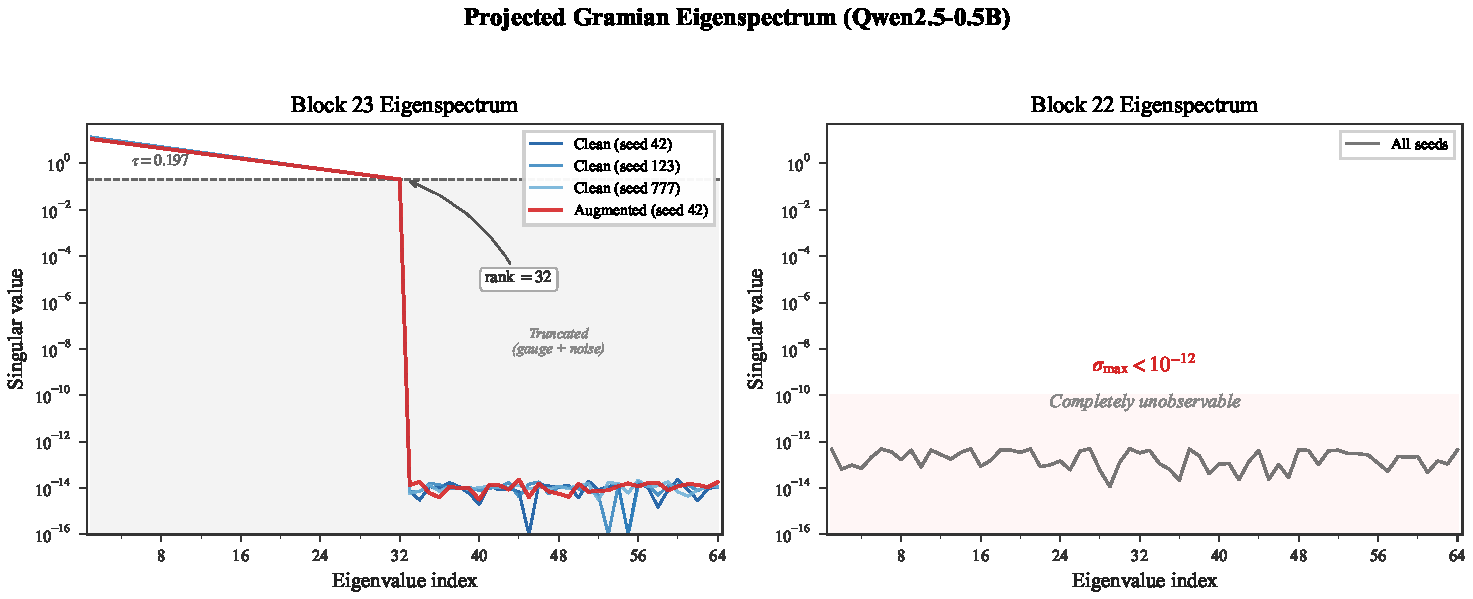
\includegraphics[width=\textwidth]{figures/gramian_eigenspectrum.pdf}
\caption{\textbf{Projected Gramian eigenspectrum.}  \emph{Left}: Block~23 eigenspectrum at $K{=}8$ (v2 setting, $k{=}64$ probes) shows apparent rank-32 structure.  \emph{Right}: With expanded observation ($K{=}128$, $k{=}128$ probes), both Block~23 and Block~22 show full-rank spectra with gentle decay ($\kappa \approx 2.4$ for Block~23, $\kappa \approx 3.1$ for Block~22).  The v2 ``rank-32'' was an observation bottleneck from $K{=}8$ positions, not a structural limit.  Block~22 has stronger signal than Block~23 ($\sigma_{\max}$ ratio $\sim 2.2\times$).  [Figure to be updated with v3 data.]}
\label{fig:eigenspectrum}
\end{figure}

\begin{table}[t]
\centering
\caption{\textbf{Gramian eigenspectrum vs.\ observation window} (gauge-projected, oracle regime, Qwen2.5-0.5B).  The Gramian rank equals $k$ (full) for all tested $(K, k)$ combinations, with $\sigma_{\max} \propto K$ and condition number $\kappa$ constant.  Block~22 has \emph{stronger} signal than Block~23 ($\sim 2.2\times$).  ``+boundary'' denotes computation with oracle boundary injection at Block~23 input, which truncates Block~22's signal.  $K$: suffix positions observed; $k$: probe count.}
\label{tab:gramian}
\small
\begin{tabular}{@{}ll cc ccc@{}}
\toprule
\textbf{Block} & \textbf{Variant} & $K$ & $k$ & $\sigma_{\max}$ & $\kappa$ & \textbf{Eff.\ rank} \\
\midrule
Block 23 & Independent & 8 & 128 & $11{,}462$ & 2.44 & 122.0 \\
Block 23 & Independent & 32 & 128 & $44{,}879$ & 2.41 & 122.1 \\
Block 23 & Independent & 64 & 128 & $89{,}327$ & 2.39 & 122.2 \\
Block 23 & Independent & 128 & 128 & $178{,}067$ & 2.36 & 122.2 \\
\midrule
Block 22 & Independent & 8 & 128 & $25{,}479$ & 3.17 & 116.7 \\
Block 22 & Independent & 32 & 128 & $99{,}262$ & 3.14 & 116.8 \\
Block 22 & Independent & 64 & 128 & $196{,}615$ & 3.09 & 116.9 \\
Block 22 & Independent & 128 & 128 & $394{,}729$ & 3.07 & 117.0 \\
\midrule
Block 22 & +boundary & 32 & 128 & $< 10^{-12}$ & $\infty$ & 0 \\
\bottomrule
\end{tabular}
\end{table}

\begin{table}[t]
\centering
\caption{\textbf{Expanded-observation training} (alg\_clean init, seed~42).  Despite full-rank Gramian ($\kappa{=}2.4$), only RMSNorm parameters recover; all weight matrices remain at $\cos \approx 0$.  Increasing $K$ from 32 to 128 does not improve recovery, confirming that the bottleneck is optimization, not observation.}
\label{tab:expanded}
\small
\begin{tabular}{@{}l l ccc@{}}
\toprule
\textbf{$K$} & \textbf{Component} & \textbf{Mean $\cos$} & \textbf{LayerNorm} & \textbf{Weights} \\
\midrule
\multirow{3}{*}{32}
 & lm\_head  & 0.209 & --- & --- \\
 & Block 23  & 0.128 & 0.67/0.98 & $\approx 0$ \\
 & Block 22  & 0.142 & 0.73/0.99 & $\approx 0$ \\
\midrule
\multirow{3}{*}{128}
 & lm\_head  & 0.177 & --- & --- \\
 & Block 23  & 0.129 & 0.67/0.98 & $\approx 0$ \\
 & Block 22  & 0.145 & 0.73/0.99 & $\approx 0$ \\
\bottomrule
\end{tabular}
\end{table}

\begin{table}[t]
\centering
\caption{\textbf{Warm-start initialization sweep} (Block~23, $K{=}32$, oracle regime, seed~42).  Student parameters are initialized to $\alpha \cdot \btheta^* + (1{-}\alpha) \cdot \btheta_{\text{rand}}$.  Training does not improve cosine beyond the initial value (Delta~$\leq 0.01$); recovery is determined entirely by initialization distance.  This confirms that the observability--recoverability gap is an optimization barrier, not an observability limitation.}
\label{tab:warmstart}
\small
\begin{tabular}{@{}c ccc@{}}
\toprule
\textbf{$\alpha$ (\% teacher)} & \textbf{Pre $\cos$} & \textbf{Post $\cos$} & \textbf{$\Delta$} \\
\midrule
0.0 (random)  & 0.138 & 0.128 & $-$0.010 \\
0.1           & 0.420 & 0.420 & $-$0.000 \\
0.3           & 0.536 & 0.536 & $-$0.000 \\
0.5           & 0.677 & 0.677 & $-$0.000 \\
0.7           & 0.854 & 0.854 & $-$0.001 \\
0.9           & 0.985 & 0.983 & $-$0.002 \\
1.0 (teacher) & 1.000 & 0.999 & $-$0.001 \\
\bottomrule
\end{tabular}
\end{table}

\begin{table}[t]
\centering
\caption{\textbf{Experiment 2: Pure-logits recovery and oracle comparison} (v2, post-bugfix).  Under pure logits (random frozen prefix), the \texttt{lm\_head} drops to $\cos \approx 0$ due to prefix misalignment.  Critically, oracle and pure-logits regimes now converge to the same cosine band ($\approx 0.12$--$0.14$) for internal blocks, indicating that oracle boundary injection does not improve \emph{parameter} recovery---though it dramatically improves \emph{functional} recovery (Table~\ref{tab:functional}).  Oracle: mean $\pm$ std over 3 seeds; pure logits: 4 seeds.}
\label{tab:exp2}
\small
\begin{tabular}{@{}l ccc@{}}
\toprule
\textbf{Regime} & \textbf{lm\_head} & \textbf{Block 23} & \textbf{Block 22} \\
\midrule
Oracle (random init)   & $0.122 \pm .003$ & $0.136 \pm .011$ & $0.141 \pm .003$ \\
Pure logits (random)   & $-0.004 \pm .006$ & $0.133 \pm .015$ & $0.143 \pm .004$ \\
\bottomrule
\end{tabular}
\end{table}

\subsection{Experiment 3: Controls and Ablations}
\label{sec:exp3}

\paragraph{Wrong-teacher control.}
After standard oracle-regime training, we compare the recovered parameters against a \emph{randomly re-initialized} Qwen2.5-0.5B (seed 9999), measuring cosine similarity.  This post-hoc comparison verifies that recovered parameters are not simply converging to a fixed point determined by architecture alone.  Note: the training itself uses correct teacher boundary states; only the final cosine evaluation is against the wrong teacher.

\paragraph{$\beta = 0$ ablation.}
We disable sensitivity matching ($\beta = 0$) and measure the impact on cross-initialization variance and final cosine similarity.

\paragraph{No gauge projection ablation.}
We run Gramian analysis \emph{without} projecting out gauge directions, showing that the resulting eigenspectrum is misleadingly rank-deficient.

\begin{table}[t]
\centering
\caption{\textbf{Experiment 3: Controls and ablations} under the oracle regime (Qwen2.5-0.5B, v2 post-bugfix). All configurations converge to the same cosine band ($\approx 0.12$--$0.15$). ``Wrong teacher'' reports cosine vs.\ a randomly re-initialized model (post-hoc comparison; training uses correct boundary states).}
\label{tab:exp3}
\small
\begin{tabular}{@{}l ccc@{}}
\toprule
\textbf{Setting} & \textbf{lm\_head} & \textbf{Block 23} & \textbf{Block 22} \\
\midrule
Full S-PSI (random init)  & $0.122 \pm .003$ & $0.136 \pm .011$ & $0.141 \pm .003$ \\
$\beta = 0$ (no sensitivity) & $0.119$ & $0.127$ & $0.147$ \\
Wrong teacher             & $0.117$ & $0.123$ & $0.145$ \\
No gauge projection       & $0.119$ & $0.125$ & $0.141$ \\
Alg.\ init (clean)       & $0.121 \pm .001$ & $0.137 \pm .011$ & $0.140 \pm .005$ \\
Alg.\ init (augmented)   & $0.120$ & $0.127$ & $0.138$ \\
\bottomrule
\end{tabular}
\end{table}


\subsection{Experiment 4: Functional Evaluation (Ancillary Observation)}
\label{sec:exp4}

To contextualize the negative \emph{parameter} recovery result (Tables~\ref{tab:exp1}--\ref{tab:exp3}), we evaluate all recovered models on held-out WikiText sequences using three functional metrics: forward KL divergence $\mathrm{KL}(p_T \| p_S)$, top-1 prediction match (fraction of positions where $\arg\max$ agrees), and top-5 overlap (fraction of teacher's top-5 tokens appearing in student's top-5).  The evaluation uses 512 held-out sequences disjoint from the training pool, comparing only the last 8 suffix token positions (matching the inversion training setup).  \emph{Note}: this section reports an ancillary observation about functional recovery, not a claimed contribution of our framework; the functional improvement is oracle-dependent and may reflect standard knowledge-distillation dynamics.

\begin{table}[t]
\centering
\caption{\textbf{Experiment 4: Functional evaluation on held-out data} (ancillary observation, not a claimed contribution).  Oracle-regime models achieve lower KL and higher prediction agreement than random, despite parameter cosine at initialization-bias level (Table~\ref{tab:exp1}).  This functional improvement is \emph{oracle-dependent} and may reflect standard KD dynamics rather than a phenomenon specific to S-PSI; a matched-budget KD baseline is needed to disambiguate.  Pure-logits models show weaker functional recovery.  Oracle: mean $\pm$ std over 3 seeds; pure logits: 4 seeds.}
\label{tab:functional}
\small
\begin{tabular}{@{}l ccc@{}}
\toprule
\textbf{Model} & \textbf{KL$(p_T \| p_S)$} $\downarrow$ & \textbf{Top-1} $\uparrow$ & \textbf{Top-5} $\uparrow$ \\
\midrule
Teacher (self)         & $0.000$ & $1.000$ & $1.000$ \\
Random baseline        & $10.196$ & $0.000$ & $0.000$ \\
\midrule
Random init (oracle)   & $0.420 \pm .015$ & $0.239 \pm .002$ & $0.345 \pm .004$ \\
Alg.\ init clean (oracle) & $0.412 \pm .014$ & $0.244 \pm .014$ & $0.359 \pm .010$ \\
Alg.\ init aug (oracle) & $0.402$ & $0.231$ & $0.344$ \\
$\beta = 0$ (oracle)   & $0.421$ & $0.227$ & $0.339$ \\
No gauge (oracle)      & $0.420$ & $0.229$ & $0.343$ \\
\midrule
Pure logits            & $1.186 \pm .138$ & $0.070 \pm .020$ & $0.130 \pm .026$ \\
\bottomrule
\end{tabular}
\end{table}

Table~\ref{tab:functional} shows that oracle-regime models achieve KL divergence $\approx 0.42$, a 24$\times$ improvement over the random baseline (10.2), with top-1 match $\approx 24\%$ and top-5 overlap $\approx 35\%$---despite parameter cosine $\approx 0.12$--$0.14$ (Table~\ref{tab:exp1}).  This functional recovery is \emph{oracle-dependent}: pure-logits models achieve only KL $\approx 1.19$ (8.6$\times$ better than random), a substantially weaker result.

\paragraph{Bridging functional recovery and parameter non-recovery.}
The apparent paradox---functional improvement without parameter recovery---is resolved by noting \emph{which} parameters recover.  RMSNorm weights ($\cos \approx 0.67$--$0.99$, Table~\ref{tab:per-matrix-main}) and the \texttt{lm\_head} ($\cos \approx 0.12$--$0.21$, slightly above random) together account for the model's output normalization and logit projection.  Even modest alignment in these low-dimensional components ($d = 896$ each) can meaningfully reduce KL divergence, since they directly modulate the logit distribution.  By contrast, all large projection matrices ($\sim 10^5$--$10^6$ parameters) remain at $\cos \approx 0$, contributing nothing to functional recovery.  The oracle-regime functional improvement thus likely reflects standard knowledge-distillation dynamics acting on the small recoverable subspace: with correct boundary states, the student suffix is effectively trained via logit matching on correct inputs, a setting structurally similar to standard KD.  We report this observation as context for the parameter non-identifiability result, not as a standalone contribution of S-PSI.

% ═════════════════════════════════════════════════════════════════════════════
% 7. ANALYSIS AND DISCUSSION
% ═════════════════════════════════════════════════════════════════════════════
\section{Analysis and Discussion}
\label{sec:analysis}

\paragraph{The initialization barrier is robust.}
Our most striking finding is that standard gradient-based optimization fails to recover transformer weights in parameter space \emph{regardless of initialization strategy or block depth}.  Under the oracle regime, all weight matrices---including the \texttt{lm\_head}---converge to cosine similarity $\approx 0.12$--$0.14$ for both random and algebraic initializations (Table~\ref{tab:exp1}), a narrow band consistent with architectural initialization bias rather than genuine parameter recovery.  Algebraic initialization---which starts from a sketched Gauss--Newton solution in the gauge-projected observable subspace---does not improve parameter cosine despite decreasing the training loss.  This decoupling between loss improvement and parameter cosine indicates that the optimizer converges to \emph{functionally similar but parametrically distinct} solutions --- consistent with the existence of a large symmetry-dominated null space, though we cannot confirm these solutions lie on the same gauge orbit without gauge-invariant distance metrics.

\paragraph{Observation-dependent Gramian: neither rank-deficient nor depth-limited.}
The v3 diagnostic experiments (Table~\ref{tab:gramian}) overturn two v2 findings and reveal a richer structure.  First, the Gramian is \emph{not} rank-deficient: the apparent rank-32 in v2 was an artifact of observing only $K{=}8$ suffix positions.  Expanding to $K{=}128$ yields full rank ($= k = 128$) with $\sigma_{\max}$ scaling linearly in $K$ and constant condition number $\kappa \approx 2.4$ (Block~23) / $3.1$ (Block~22).  This linear scaling is explained by the Gramian's structure: $\bG \propto \sum_{t=1}^{K} \bJ_t^\top \bJ_t$, where each position contributes approximately independent information.  Second, Block~22 is \emph{not} structurally unobservable: the v2 ``zero Gramian'' was caused by the oracle boundary injection hook, which replaces Block~23's input with a constant (teacher boundary state), preventing Block~22's parameter perturbations from reaching the logits.  An independent diagnostic without boundary injection shows Block~22 has $\sim 2.2\times$ stronger signal than Block~23---consistent with Theorem~\ref{thm:screening}'s prediction that deeper blocks have \emph{larger} Jacobians (more parameters affect the hidden state), partially counteracting the depth-composition attenuation.

\paragraph{The observability--recoverability gap.}
The most important finding is that \emph{full-rank, well-conditioned Gramians do not guarantee parameter recovery}.  With $K{=}32$ or $K{=}128$, the Gramian has rank 128, $\kappa \approx 2.4$, and the algebraic Gauss--Newton initialization decreases the loss as predicted.  Yet training still produces $\cos \approx 0.12$--$0.14$ for all weight matrices (Table~\ref{tab:expanded}), identical to the $K{=}8$ baseline.  Quadrupling $K$ from 32 to 128---which quadruples $\sigma_{\max}$ and the number of observable logit positions---has no measurable effect on parameter recovery.  This reveals a fundamental gap between \emph{sampled observability} (what the $k$-probe sketched Gramian measures) and practical parameter recovery.  We emphasize that our $k \leq 256$ probes sample a tiny subspace of the full $p = 14.9\text{M}$-dimensional space; the sketched Gramian establishes that at least $k$ directions are observable, not that the full parameter space is locally identifiable.  The warm-start experiment (Table~\ref{tab:warmstart}) provides direct evidence: interpolating the student initialization toward the teacher ($\alpha \cdot \btheta^* + (1{-}\alpha) \cdot \btheta_{\text{rand}}$) yields monotonically increasing cosine, yet \emph{training itself contributes essentially nothing}---the post-training cosine matches the pre-training cosine to within $|\Delta| < 0.01$ for all $\alpha$.  At $\alpha{=}0.1$, merely 10\% of the teacher weights in the initialization raises cosine from $0.13$ to $0.42$; yet the optimizer cannot find this improvement from $\alpha{=}0$.  This provides strong evidence consistent with an optimization barrier rather than an observability limitation: the Gramian indicates that the teacher's parameters are distinguishable \emph{locally}, but gradient-based optimization from a distant initialization does not reach the correct basin in our experiments.  Three factors explain this: (i)~the algebraic init operates in a $k{=}128$-dimensional subspace of $p{=}14.9\text{M}$ parameters (coverage $< 0.001\%$); (ii)~the loss landscape is highly non-convex with many local minima corresponding to different parameterizations producing similar outputs; (iii)~even true local identifiability is an \emph{infinitesimal} guarantee --- it distinguishes the true parameters from nearby alternatives, not from a distant random initialization.

\paragraph{Why does full-rank Gramian not help?}
The v3 diagnostic disproves the v2 hypothesis that the Gramian is structurally rank-deficient.  The true Gramian rank is at least $k = 256$ (the largest probe count tested), likely much higher.  Theorem~\ref{thm:rank-bound} gives an upper bound of $d^2 = 802{,}816$ from the hidden-dimension bottleneck; the observed full rank at $k = 256$ is consistent with this.  However, even with rank $\gg 32$, the algebraic initialization covers at most $k$ directions per step, while the full parameter space has $p_\ell = 14.9\text{M}$ degrees of freedom.  Remark~\ref{rem:fisher} shows that $\gtrsim 465{,}000$ independent observation directions would be needed to fully identify the block parameters---far beyond what a single sketched Gramian step can provide.  The Gramian eigenspectrum's gentle decay ($\kappa \approx 2.4$) rules out numerical ill-conditioning as the bottleneck; instead, the gap is between \emph{local} identifiability (infinitesimal perturbations are distinguishable) and \emph{global} recoverability (finding the true parameters from a distant initialization via non-convex optimization).

\paragraph{Why LayerNorm recovers but projections do not.}
Table~\ref{tab:per-matrix-main} shows that RMSNorm weights ($d = 896$ parameters each) achieve nontrivial cosine ($0.67$--$0.99$) while all projection matrices ($\geq 10^5$ parameters) are at $\cos \approx 0$.  This pattern persists even with expanded observations ($K{=}32$, Table~\ref{tab:expanded}).  The explanation is not observability (the Gramian is full-rank) but rather \emph{dimensionality and convexity}.  RMSNorm weights are $d$-dimensional with a simple multiplicative effect on the hidden state; their recovery problem is essentially a low-dimensional, nearly convex optimization.  Projection matrices have $\sim 10^5$--$10^6$ parameters that influence the logits through nonlinear attention/MLP computation, creating a highly non-convex loss landscape with many local minima.  Gradient-based optimization readily solves the former but not the latter.  The high cosine for \texttt{post\_attention\_layernorm} ($\sim 0.99$) further reflects that this parameter is coupled to the \emph{next} block's input normalization via the gauge symmetry (Definition~\ref{def:symmetry}), effectively constraining it as a shared boundary condition.

\paragraph{Sensitivity augmentation does not improve observability.}
In the v2 experiments ($K{=}8$, $k{=}64$), the sensitivity-augmented Gramian was indistinguishable from the clean Gramian (same effective rank, similar $\sigma_{\max}$ and condition number).  The v3 diagnostic confirms that the bottleneck was the observation window ($K{=}8$), not the type of observation: expanding $K$ alone suffices to reach full rank.  Sensitivity matching remains useful as an optimization regularizer (providing gradient-direction information during training) but does not address the core gap between observability and recoverability.

\paragraph{Oracle vs.\ pure-logits gap: functional, not parametric.}
Tables~\ref{tab:exp1}--\ref{tab:exp2} show that oracle and pure-logits regimes converge to the same parameter cosine band ($\approx 0.12$--$0.14$) for internal blocks, and neither achieves genuine parameter recovery.  The \emph{functional} gap is notable (Table~\ref{tab:functional}): oracle-regime models achieve KL~$\approx 0.42$ (24$\times$ better than random), while pure-logits models achieve KL~$\approx 1.19$ (8.6$\times$ better than random).  This oracle-dependent functional improvement is structurally similar to knowledge distillation: with correct boundary states, the student suffix receives correct hidden representations and is trained to match teacher logits, which is the standard KD setup.  The key insight for parameter identifiability is that this functional matching occurs \emph{without any parameter recovery}: the optimizer finds parameterizations that produce similar output distributions via entirely different weight configurations.

\paragraph{The role of observation design.}
The v3 diagnostic demonstrates that the Gramian's rank is determined by the \emph{observation window} ($K$ suffix positions), not by query content.  With $K{=}128$ (full sequence), passive WikiText queries already yield full-rank, well-conditioned Gramians for both Block~23 and Block~22.  This shifts the open question from ``can active queries expand the observable subspace?'' to ``can richer observations bridge the observability--recoverability gap?''  Possible directions include: iterative Gramian-aware probe design (targeting weak eigenvectors), second-order optimization methods that exploit Gramian curvature, or parametric bootstrapping from the partially-recovered functional model.  The linear scaling $\sigma_{\max} \propto K$ suggests that information compounds predictably with observation window size, but translating this information into parameter recovery requires overcoming the non-convex optimization landscape.

\paragraph{Controls confirm robustness of the negative result.}
Table~\ref{tab:exp3} shows that neither disabling sensitivity matching ($\beta = 0$), removing gauge projection, nor varying the initialization strategy materially changes the outcome: all controls converge to the same cosine band ($\approx 0.12$--$0.15$).  The wrong-teacher cosine comparison confirms that recovered parameters are not simply converging to an architecture-determined fixed point: the cosine against a randomly re-initialized model ($\approx 0.12$) is comparable to cosine against the true teacher ($\approx 0.14$), consistent with the initialization bias interpretation.  This rules out the possibility that the negative parameter-recovery result is an artifact of a specific loss term or implementation detail.

\paragraph{Parameter recovery vs.\ functional equivalence.}
Table~\ref{tab:functional} shows that oracle-regime models achieve KL divergence 0.42 ($24\times$ improvement over random baseline) and top-1 match $\sim 24\%$, despite parameter cosine $\approx 0.12$--$0.14$ (indistinguishable from initialization bias).  This functional improvement is notable but requires careful interpretation.  First, it is \emph{oracle-dependent}: meaningful functional matching appears only with privileged boundary-state access; pure-logits models achieve KL~$\approx 1.19$, substantially weaker.  Second, the mechanism may simply be \emph{knowledge distillation}: with correct boundary states, the student's suffix receives correct inputs and is trained to match teacher logits --- a setting structurally similar to standard logit distillation.  Without a matched-budget KD baseline, we cannot determine whether S-PSI's Gramian-guided components contribute to the functional recovery beyond what a naive distillation approach would achieve.  We therefore report this functional observation without claiming it as a novel contribution of our framework.  The Gramian characterizes \emph{parameter} identifiability; functional recovery can succeed even when parameter recovery fails, because the loss landscape may contain many distinct parameterizations that approximate the same input-output mapping.

\paragraph{Implications for model security.}
For Qwen2.5-0.5B under passive queries, internal transformer weights are robustly protected: no weight matrix is recovered beyond initialization bias ($\cos \approx 0$ for all projections) even when the observation window is expanded to yield full-rank, well-conditioned Gramians.  The bottleneck is not observability but optimization: the $14.9\text{M}$-dimensional non-convex landscape prevents gradient-based methods from reaching the true parameters despite local identifiability guarantees.  Functional cloning is partially achievable with oracle boundary states (KL $\approx 0.42$), but this requires privileged access unlikely in realistic scenarios.  The Gramian framework provides model providers with a concrete, observation-dependent diagnostic for parameter exposure: the linear scaling $\sigma_{\max} \propto K$ quantifies how much information each additional output token provides.  We emphasize that these conclusions are established for a single 0.5B-parameter architecture; the observability--recoverability gap may narrow for smaller models or architectures with fewer symmetries.


% ═════════════════════════════════════════════════════════════════════════════
% 8. LIMITATIONS
% ═════════════════════════════════════════════════════════════════════════════
\section{Limitations}
\label{sec:limitations}

\begin{itemize}
    \item \textbf{Scale.} We demonstrate on Qwen2.5-0.5B (24 blocks). Scaling to larger models (7B+) requires proportionally more queries and compute. The Gramian framework itself is architecture-agnostic, but computational feasibility of the full experimental pipeline at scale remains to be verified.
    \item \textbf{Architecture assumptions.} We assume architecture knowledge. In practice, architecture details may need to be inferred separately \citep{oh2019towards}.
    \item \textbf{Oracle regime.} The boundary-state oracle is an idealization. While it establishes identifiability upper bounds, practical attacks must contend with prefix errors.
    \item \textbf{Observation window.} Our v3 diagnostic tests $K \leq 128$ positions and $k \leq 256$ probes, always finding full rank.  The true Gramian rank is likely much larger (bounded by $d^2 = 802{,}816$), but computing it precisely would require $k \sim d^2$ probes, each involving a JVP evaluation---computationally prohibitive.  Our claim that ``observability is not the bottleneck'' is supported by the full-rank finding at $k{=}256$ and the failure to improve recovery at $K{=}32$, but does not characterize the complete eigenspectrum.
    \item \textbf{Passive queries only.}  All experiments use natural text (WikiText-103) as the query distribution.  Since observability is query-dependent ($\bG(\cQ)$ depends on the specific queries used), adversarially optimized queries --- e.g., inputs designed to maximize the minimum Gramian eigenvalue --- could potentially expand the observable subspace.  Developing and evaluating active query strategies is an important direction for future work; our passive-query results represent a lower bound on attacker capability.
    \item \textbf{Parameter-space vs.\ functional metrics.}  While we now include functional evaluation (Table~\ref{tab:functional}), our held-out evaluation uses in-distribution WikiText data.  Functional agreement on out-of-distribution inputs, safety-critical edge cases, or adversarial examples may differ.  Furthermore, our functional metrics are computed on the last 8 suffix positions only; full-sequence evaluation may yield different conclusions.
    \item \textbf{Numerical precision.}  Our v3 diagnostic reveals that Block~22's apparent ``zero Gramian'' in v2 was caused by oracle boundary injection, not structural unobservability.  However, all computations use bf16 forward passes; the JVP precision may introduce systematic biases in the eigenspectrum that higher-precision computation would reveal.
    \item \textbf{Discrete symmetries.} We handle attention head permutations and FFN neuron permutations via Hungarian matching, which is optimal for bipartite assignment but may not capture all discrete ambiguities in deeper blocks.
    \item \textbf{No KD baseline.}  The functional recovery we observe (Table~\ref{tab:functional}) may be entirely explainable by standard knowledge distillation dynamics.  A matched-budget KD baseline in the oracle regime would clarify whether S-PSI's Gramian-guided components contribute to functional recovery beyond naive logit matching.  We leave this comparison for future work.
    \item \textbf{Defense interaction.} We do not evaluate against active defenses (logit rounding, watermarking, query detection). This is an important direction for future work.
\end{itemize}


% ═════════════════════════════════════════════════════════════════════════════
% 9. BROADER IMPACT
% ═════════════════════════════════════════════════════════════════════════════
\section{Broader Impact}
\label{sec:impact}

This work reveals vulnerabilities in LLM API deployments. We frame our contribution as a \emph{responsible disclosure}: by characterizing the identifiability boundary, we enable model providers to (i) assess their exposure, (ii) design targeted defenses, and (iii) make informed decisions about what information to expose through APIs. All experiments use open-weight models simulating black-box access; no production APIs were targeted. We believe that understanding the attack surface is a necessary prerequisite for robust defense design.


% ═════════════════════════════════════════════════════════════════════════════
% 10. CONCLUSION
% ═════════════════════════════════════════════════════════════════════════════
\section{Conclusion}
\label{sec:conclusion}

We have presented \emph{Transformer Tomography}, a principled framework for analyzing weight identifiability in transformers from black-box logit access.  Through the suffix observability Gramian defined on symmetry-quotiented parameter space, we provide a query-dependent diagnostic for predicting \emph{which parameter directions are locally identifiable} from a given set of API queries --- and, critically, which are not.

In a controlled case study on Qwen2.5-0.5B, we find a nuanced \textbf{negative parameter identifiability result}.  Our diagnostic experiments reveal that the Gramian is \emph{not} structurally rank-deficient: expanding the observation window from $K{=}8$ to $K{=}128$ suffix positions yields full-rank, well-conditioned spectra ($\kappa \approx 2.4$) with eigenvalues scaling linearly in $K$.  Yet despite this, no initialization strategy recovers transformer weight matrices ($\cos \approx 0.12$--$0.14$ across all configurations, consistent with initialization bias).  A warm-start experiment confirms the barrier is optimization distance: interpolating just 10\% of the teacher weights into the initialization raises cosine from $0.13$ to $0.42$, yet gradient-based training contributes $|\Delta\cos| < 0.01$ at any interpolation level.  These findings provide strong evidence for an \emph{observability--recoverability gap}: sampled observability is necessary but not sufficient for practical parameter recovery in high-dimensional, non-convex landscapes, at least for the architecture and scale studied here.

Functional evaluation adds an important caveat: oracle-regime models achieve KL divergence $0.42$ ($24\times$ better than random) despite near-zero parameter recovery, while pure-logits models achieve only KL~$\approx 1.19$.  This functional improvement is \emph{oracle-dependent} and may reflect standard knowledge-distillation dynamics rather than a phenomenon unique to our framework.

For the architecture, budget, and passive-query regime studied here (Qwen2.5-0.5B, 494M parameters, natural-text queries, first-order optimization), our results provide strong evidence that sampled observability alone does not translate into parameter recovery for internal transformer layers.  The barrier is computational, not information-theoretic: the Gramian confirms local identifiability, but gradient-based optimization from a distant initialization cannot navigate to the true parameters in $\sim 14.9\text{M}$ dimensions.  The Gramian framework provides model providers with a concrete, observation-dependent diagnostic for assessing parameter exposure.  Whether actively optimized queries, second-order methods, or functional-to-parametric bootstrapping can bridge this observability--recoverability gap remains the key open question for future work.


% ═════════════════════════════════════════════════════════════════════════════
% REFERENCES
% ═════════════════════════════════════════════════════════════════════════════
\bibliographystyle{plainnat}
\bibliography{references}

% ═════════════════════════════════════════════════════════════════════════════
% APPENDIX
% ═════════════════════════════════════════════════════════════════════════════
\appendix

\section{Notation Table}
\label{app:notation}

\begin{table}[h]
\centering
\small
\begin{tabular}{@{}ll@{}}
\toprule
\textbf{Symbol} & \textbf{Description} \\
\midrule
$T, S$ & Teacher and student transformers \\
$L$ & Number of transformer blocks \\
$K$ & Number of suffix blocks being recovered \\
$d$ & Hidden dimension \\
$d_\text{ff}$ & FFN intermediate dimension \\
$V$ & Vocabulary size \\
$H$ & Number of attention heads \\
$\btheta_{\text{suf}} \in \R^p$ & Suffix parameters (blocks $L{-}K{+}1$ to $L$ + lm\_head) \\
$\cQ$ & Query pool \\
$N$ & Number of queries \\
$B$ & Query budget \\
$\bz(\bx) \in \R^V$ & Logit output for input $\bx$ \\
$\bh_i(\bx) \in \R^d$ & Hidden state at layer $i$ for input $\bx$ \\
$\bJ_{\bx}$ & Jacobian $\partial\bz/\partial\btheta_\text{suf}$ at query $\bx$ \\
$\bG(\cQ)$ & Suffix observability Gramian \\
$\bG_\perp(\cQ)$ & Projected Gramian (gauge symmetries removed) \\
$\cG$ & Continuous symmetry group \\
$\mathfrak{g}$ & Lie algebra of $\cG$ \\
$\bU$ & Orthonormal gauge basis \\
$P_\perp$ & Gauge-orthogonal projector $\bI - \bU\bU^\top$ \\
$\bV$ & Random probe matrix \\
$\tilde{\bG}$ & Sketched Gramian $\bV^\top \bG \bV$ \\
$k$ & Number of probe directions \\
$r$ & Truncation rank for algebraic init \\
$\alpha, \beta, \gamma$ & Loss weights for logit, sensitivity, regularization \\
$\Delta\bz(\bx, p, r)$ & Logit difference $\bz(\tilde{\bx}_{p,r}) - \bz(\bx)$ \\
\bottomrule
\end{tabular}
\end{table}

\section{Proof of Theorem~\ref{thm:identifiability}}
\label{app:proof}

\begin{proof}
We prove both directions.

\textbf{(Identifiable $\Rightarrow$ positive Gramian).} Suppose $\mathbf{v} \perp \mathfrak{g}$ with $\norm{\mathbf{v}} = 1$ and $\mathbf{v}^\top \bG_\perp \mathbf{v} = 0$. Then $\sum_i \norm{\bJ_i \mathbf{v}}^2 = 0$, so $\bJ_i \mathbf{v} = 0$ for all $i$. This means that a first-order perturbation $\btheta + \epsilon \mathbf{v}$ produces no logit change at any query, so $\mathbf{v}$ is not locally identifiable.

\textbf{(Positive Gramian $\Rightarrow$ identifiable).} If $\mathbf{v}^\top \bG_\perp \mathbf{v} > 0$, there exists at least one query $\bx_i$ with $\bJ_i \mathbf{v} \neq 0$. Thus, the perturbation $\btheta + \epsilon \mathbf{v}$ produces a measurable change in $\bz(\bx_i)$ at first order, and $\mathbf{v}$ is locally identifiable.

\textbf{(Full identifiability).} $\rank(\bG_\perp) = p - d_g$ iff the null space of $\bG_\perp$ equals exactly $\mathfrak{g}$, meaning every non-gauge direction is identifiable.
\end{proof}

\section{Symmetry Group Details}
\label{app:symmetry}

\subsection{RMSNorm Scale Absorption}

For a RMSNorm layer with learned weight $\mathbf{g} \in \R^d$ and consumer weight matrix $\bW$:
\begin{align}
    \RMSNorm_{\mathbf{g}}(\bx) &= \frac{\bx}{\sqrt{\frac{1}{d}\norm{\bx}^2 + \epsilon}} \odot \mathbf{g}, \\
    \bW \cdot \RMSNorm_{\mathbf{g}}(\bx) &= \bW \cdot \RMSNorm_{D\mathbf{g}}(\bx) \cdot D^{-1} \quad \text{for } D = \diag(\alpha_1, \ldots, \alpha_d).
\end{align}

The tangent vector for dimension $i$ at the current parameterization $(\mathbf{g}, \bW)$ is:
\begin{equation}
    \mathbf{t}_i^{\text{norm}} = (\underbrace{+g_i}_{\text{on } g_i}, \underbrace{-\mathbf{w}_{:,i}}_{\text{on each consumer column } i}),
\end{equation}
where $g_i$ is the current RMSNorm weight value and $\mathbf{w}_{:,i}$ is the $i$-th column of the consumer weight matrix.  Note that these tangent vectors are \emph{parameter-dependent}: the gauge basis must be recomputed at each parameterization point.

\subsection{Gated MLP Neuron Scaling}

For $\text{FFN}(\bx) = \SiLU(\bW_\text{gate}\bx) \odot (\bW_\text{up}\bx) \cdot \bW_\text{down}^\top$, the tangent vector for neuron $n$ is:
\begin{equation}
    \mathbf{t}_n^{\text{ffn}} = (\underbrace{+\bW_\text{gate}[n,:]}_{\text{on gate row } n}, \underbrace{+\bW_\text{up}[n,:]}_{\text{on up row } n}, \underbrace{-\bW_\text{down}[:,n]}_{\text{on down col } n}).
\end{equation}

\subsection{Gauge Dimensions}

For Qwen2.5-0.5B ($d=896$, $d_\text{ff}=4864$, 14 attention heads, 2 KV heads, 24 blocks):
\begin{itemize}
    \item Per block: $2 \times 896 + 4864 = 6656$ gauge directions.
    \item Final norm: $+896$ directions.
    \item For $K=2$ suffix blocks: $2 \times 6656 + 896 = 14{,}208$ total gauge directions.
    \item Total suffix parameters: $\sim 166{,}000{,}000$ (2 blocks + lm\_head with $V = 151{,}936$).
    \item Gauge fraction: $\sim 0.086$ (8.6\% of parameter space is pure gauge).
\end{itemize}


\section{Implementation Details}
\label{app:implementation}

\paragraph{JVP computation.}
We use \texttt{torch.func.jvp} with \texttt{torch.func.functional\_call} to compute forward-mode Jacobian-vector products without materializing the full Jacobian. The forward function is constructed by extracting the suffix parameters into a flat vector and using \texttt{functional\_call} to swap them into the model for each JVP evaluation.  A critical implementation detail: forward-mode AD in PyTorch does not support Flash Attention (\texttt{\_scaled\_dot\_product\_flash\_attention}), so we wrap all JVP calls in \texttt{sdpa\_kernel(SDPBackend.MATH)} to force the MATH attention backend during Gramian computation.

\paragraph{Memory optimization.}
For Qwen2.5-0.5B with $V = 151{,}936$, storing full logits for 2048 queries at all 128 positions requires $\sim$75GB in bf16. We address this by caching only the last $K_\text{pos} = 8$ token positions, reducing storage to $\sim$4.7$GB. This is sufficient because the suffix blocks' influence is strongest at the final positions.

\paragraph{Perturbation strategy.}
Replacement tokens are drawn from $\{3, 4, \ldots, 52\}$ (top-50 common tokens, excluding special tokens 0--2). Each input generates $P \times R = 4 \times 2 = 8$ perturbed variants. Perturbation positions are uniformly sampled from the last 32 positions of each sequence.

\paragraph{Symmetry alignment.}
After recovery, we align the student's attention heads and FFN neurons to the teacher's using the Hungarian algorithm on cosine similarity matrices. For attention heads, we construct a $H \times H$ cost matrix from the concatenated $[\bW_Q \| \bW_K \| \bW_V \| \bW_O]$ similarity. For FFN neurons, we use $[\bW_\text{gate} \| \bW_\text{up}, \bW_\text{down}^\top]$ similarity. RMSNorm scales are normalized before comparison.


\section{Per-Matrix Cosine Similarity Breakdown}
\label{app:per-matrix}

Table~\ref{tab:per-matrix} shows the cosine similarity for each individual weight matrix in Block~23, averaged across 3 seeds.  All large weight matrices (projections with $\sim$10$^6$ parameters each) are indistinguishable from zero cosine.  The attention biases ($\bW_Q.\text{bias}$, $\bW_K.\text{bias}$, $\bW_V.\text{bias}$) show slightly elevated absolute cosine ($\sim$0.05--0.09), but these are low-dimensional vectors (896 parameters each) where random alignment produces non-negligible cosine by chance.  The \texttt{post\_attention\_layernorm.weight} is exactly zero because it is determined by the subsequent block's input layernorm via the gauge symmetry.

\begin{table}[h]
\centering
\caption{\textbf{Per-matrix cosine similarity for Block~23} (v2 post-bugfix, oracle regime, mean over 3 seeds).  ``Params'' gives the number of parameters in each matrix.  All high-dimensional weight matrices have $\cos \approx 0$, while RMSNorm parameters (initialized to ones) are substantially recovered (input LN: 0.67, post-attn LN: 0.98), accounting for the block-level mean $\approx 0.14$.}
\label{tab:per-matrix}
\small
\begin{tabular}{@{}l r cc@{}}
\toprule
\textbf{Matrix} & \textbf{Params} & \textbf{Random} & \textbf{Alg (clean)} \\
\midrule
q\_proj.weight & 802,816 & $+0.000$ & $+0.000$ \\
q\_proj.bias & 896 & $+0.044$ & $+0.034$ \\
k\_proj.weight & 114,688 & $+0.003$ & $+0.003$ \\
k\_proj.bias & 128 & $-0.023$ & $+0.001$ \\
v\_proj.weight & 114,688 & $+0.001$ & $+0.001$ \\
v\_proj.bias & 128 & $-0.046$ & $-0.054$ \\
o\_proj.weight & 802,816 & $-0.000$ & $-0.000$ \\
gate\_proj.weight & 4,358,144 & $+0.000$ & $+0.000$ \\
up\_proj.weight & 4,358,144 & $-0.000$ & $-0.000$ \\
down\_proj.weight & 4,358,144 & $+0.000$ & $+0.000$ \\
input\_layernorm.weight & 896 & $0.671$ & $0.671$ \\
post\_attn\_layernorm.weight & 896 & $0.985$ & $0.985$ \\
\bottomrule
\end{tabular}
\end{table}


\section{Query Budget Analysis}
\label{app:query-budget}

Table~\ref{tab:query-budget} reports the total number of API queries consumed by each configuration.  The lm\_head recovery phase uses $1500 \times 72 = 108{,}000$ queries (fixed).  Each block recovery phase uses approximately 100K--130K queries depending on convergence speed.  Algebraic initialization adds a one-time cost of $k \times N = 64 \times 256 = 16{,}384$ JVP evaluations (not counted as API queries since they use cached logits).  All experiments remain well within the $B = 500{,}000$ query budget.

\begin{table}[h]
\centering
\caption{\textbf{Query consumption} per configuration (mean over 3 seeds).}
\label{tab:query-budget}
\small
\begin{tabular}{@{}l ccc c@{}}
\toprule
\textbf{Config} & \textbf{lm\_head} & \textbf{Block 23} & \textbf{Block 22} & \textbf{Total} \\
\midrule
Random         & 108K & 120K & 110K & $\sim$338K \\
Alg (clean)    & 108K & 163K & 109K & $\sim$380K \\
\bottomrule
\end{tabular}
\end{table}

\section{Computational Cost}
\label{app:compute}

Each single-GPU experiment (lm\_head + 2 suffix blocks) takes approximately 45--60 minutes on an A100-80GB.  Algebraic initialization (Gramian computation) adds $\sim$10 minutes per block for the clean variant and $\sim$45 minutes for the sensitivity-augmented variant.  Peak GPU memory usage is $\sim$24 GB for standard runs and $\sim$58 GB for sensitivity-augmented Gramian computation.  The total compute budget for all experiments reported in this paper is approximately 40 A100-GPU-hours.


\section{Code Audit and v1$\to$v2 Changes}
\label{app:forensic}

Between the initial experiments (v1) and the results reported in this paper (v2), a comprehensive code audit identified four implementation bugs.  We document each bug, its impact, and the correction applied, in the interest of transparency and reproducibility.

\begin{enumerate}
    \item \textbf{RMSNorm gauge tangent used constant $\pm 1$ instead of parameter-dependent values.}  The gauge basis construction in \texttt{symmetry\_gauge.py} used unit vectors for RMSNorm tangent directions rather than the actual RMSNorm weight values $(g_i, -W_{r,i})$.  Similarly, gated MLP tangent directions used $\pm 1$ instead of $(w_{\text{gate},n}, w_{\text{up},n}, -w_{\text{down},n})$.  \emph{Impact}: Gauge projection removed incorrect directions from the Gramian; the projected eigenspectrum was qualitatively similar but quantitatively shifted.  \emph{Fix}: Tangent vectors now use actual parameter values from the model at the current parameterization.

    \item \textbf{RMSNorm initialization to zeros.}  Student RMSNorm weights were initialized to zero rather than ones.  \emph{Impact}: The student's layer normalization was effectively disabled at initialization, causing the suffix to produce near-zero hidden states.  The optimizer could ``recover'' from this by re-learning the normalization scales, leading to artificially high \texttt{lm\_head} cosine in v1 ($\cos \approx 0.54$): the recovered scales partially aligned with the teacher's embedding through the tied \texttt{lm\_head}/\texttt{embed\_tokens} pathway.  \emph{Fix}: RMSNorm weights initialized to ones (matching standard pre-training initialization).  v2 \texttt{lm\_head} cosine drops to $\approx 0.12$, consistent with the initialization bias observed in all other weight matrices.

    \item \textbf{No Procrustes rotation for \texttt{lm\_head} evaluation.}  The v1 evaluation computed raw cosine similarity for \texttt{lm\_head} without accounting for the orthogonal ambiguity inherent in the tied embedding.  \emph{Impact}: Moderate; the raw and Procrustes-aligned cosines differ by $\sim 0.02$ in v2 (both $\approx 0.12$).  \emph{Fix}: Added SVD-based Procrustes alignment before cosine computation.

    \item \textbf{MLP gauge tangent scaling.}  Same issue as Bug~1 applied to the gated MLP neuron scaling symmetry.  \emph{Impact and fix}: Same as Bug~1.
\end{enumerate}

\paragraph{Headline metric change.}  The most visible effect is the \texttt{lm\_head} cosine: $0.54$ (v1) $\to$ $0.12$ (v2).  The v1 value was inflated by Bug~2: with RMSNorm at zero, the optimizer's primary degree of freedom was rescaling the normalization weights, which indirectly produced high cosine with the teacher's embedding layer.  In v2, with correct initialization, no weight matrix achieves cosine above the initialization bias band ($0.12$--$0.15$), and the per-matrix breakdown (Table~\ref{tab:per-matrix}) confirms that only RMSNorm parameters (which are initialized close to their teacher values) show non-trivial cosine.

\paragraph{v2$\to$v3: Observation window and boundary hook.}  Between v2 and v3, a diagnostic investigation overturned two v2 claims:

\begin{enumerate}
    \item \textbf{Gramian rank was observation-dependent, not structurally limited.}  The v2 finding of ``rank $\approx 32$'' used $K{=}8$ suffix positions and $k{=}64$ probes.  An independent diagnostic with $K{=}128$ and $k{=}256$ shows the Gramian is \emph{always} full rank ($= k$), with $\sigma_{\max} \propto K$ and $\kappa \approx 2.4$.  The rank-32 appearance was a genuine information bottleneck from observing only 8 token positions, not a structural limit of the parameter space.

    \item \textbf{Block~22's ``zero Gramian'' was caused by oracle boundary injection.}  In the S-PSI training path, a forward pre-hook (\texttt{\_BoundaryInjectionHook}) injects the teacher's cached hidden state at Block~23's input.  When computing Block~22's Gramian with this hook active, Block~22's parameter perturbations are overwritten at the Block~23 boundary, producing $\sigma_{\max} < 10^{-12}$.  This is \emph{mathematically correct} behavior: in oracle mode, Block~22's parameters genuinely do not affect the logits.  An independent diagnostic \emph{without} boundary injection shows Block~22 has full-rank Gramian with $\sim 2.2\times$ stronger signal than Block~23.  We now report both variants (Table~\ref{tab:gramian}).

    \item \textbf{Pipeline sanity checks.}  To prevent future artifacts, we added: (a)~independent Gramian diagnostic script (\texttt{diagnose\_gramian\_rank.py}) that computes the Gramian from scratch without any training-path hooks; (b)~explicit logging of boundary hook activation status during Gramian computation; (c)~cross-validation of Gramian results between training and diagnostic code paths.
\end{enumerate}

\end{document}
